\documentclass[10pt]{beamer}

%%%
% PREAMBLE FOR THIS DOC 
%%%
%https://tex.stackexchange.com/questions/68821/is-it-possible-to-create-a-latex-preamble-header
\usepackage{/Users/miw267/Repos/csci246_spring2025/slides/preambles/beamer_preamble_for_CSCI246}



%%% TRY TO RESHOW TOC AT EACH SECTION START (with current section highlighted)
% Reference: https://tex.stackexchange.com/questions/280436/how-to-highlight-a-specific-section-in-beamer-toc
\newcommand\tocforsect[2]{%
  \begingroup
  \edef\safesection{\thesection}
  \setcounter{section}{#1}
  \tableofcontents[#2,currentsection]
  \setcounter{section}{\safesection}
  \endgroup
}


%%%% HERES HOW TO DO IT CORRECTLY
% FIRST IN .STY FILE, DO
%\usetheme[sectionpage=none]{metropolis}
% THEN AT EACH SECTION DO
%\begin{frame}{Outline}
%  \tableofcontents[currentsection]	
%\end{frame}



%\setbeamertemplate{navigation symbols}{}
%\setbeamertemplate{footline}[frame number]{}


%%%
% DOCUMENT
%%%

\begin{document}

%\maketitle

%% Title page frame
%\begin{frame}
%    \titlepage 
%\end{frame}





\title{01/29/2025: Multiple Proofs}
\author{CSCI 246: Discrete Structures}
\date{Textbook reference: Ch. 2, Hampkins}

\begin{frame}
    \titlepage 
\end{frame}


\begin{frame}
\footnotesize 
\begin{myredbox}[title=Brightspace announcement highlights]
\begin{itemize}
\item Friday's problems quiz will only cover Secs. 5\,\&\,6 (Proofs \,\&\, Counterexamples). Some of today's material will be relevant to Proofs. 
\item Starting tomorrow,  Joyce Kelly's office hours are Thursdays 4-6 pm.
\end{itemize}
\end{myredbox}
\vfill 

\begin{mygreenbox}[title=New quiz return method]
Quizzes are grouped into four bins (A-G, H-L, M-R, S-Z) by last name. \\
The quizzes are upside down with your last name on the back. \\
Come find yours before, during, or after class. \\
Only turn the quiz over if it's yours.
\end{mygreenbox} 
\vfill 

\begin{myyellowbox}[title=Today's Agenda]

\begin{itemize}
	\item Reading quiz  (5 mins)
	\item Mini-lecture ($\approx$ 15 mins)
	%
	\begin{itemize}
	\footnotesize 
	\item Additional proofs practice (via Hamkins).
	\item Resolving a puzzle	 from earlier
	\end{itemize}
	%
	\item Group exercises ($\approx$ 30 mins)
	%
	\begin{itemize}
	\footnotesize 
	\item Continue the Boolean Algebra exercises.
	\end{itemize}
	%	
\end{itemize}

\end{myyellowbox}
\vfill 


\end{frame}




\begin{frame}{Reading Quiz}

\begin{myyellowbox}[title=Logistics Alert]
Please setup your quizzes in the standard way, but \textbf{also} write your last name on the back of the page. 
\end{myyellowbox}
\vfill
 \begin{mygreenbox}[title=Reading Quiz (Multiple Proofs - Hampkins CH 2)]
Use one of the seven methods in the textbook, or perhaps your own method, to prove the theorem below.  For \texttt{extra credit}, provide two different proofs. \\

\textbf{Theorem.} \textit{For any natural number $n$, the number $n^2-n$ is even.}
\end{mygreenbox}
\vfill 

\begin{myredbox}[title=Definition]
The \textbf{natural numbers} are the non-negative integers: $0,1,2,3, \hdots$.
\end{myredbox}


\end{frame}






\begin{frame}{Multiple Proofs}

\begin{mygreenbox}[title=Quote of the Day]
“Perhaps the greatest pleasure of mathematics is that, as you try to solve problems, you find that you come to understand new techniques. You see the problem \textbf{from a different perspective}, and that’s when you make progress.”  \\

-- Andrew Wiles (who famously solved Fermat's Last Theorem)
\end{mygreenbox}
	
\vfill \vfill 
\begin{myredbox}[title=Role of this chapter]
\begin{itemize}
\item To demonstrate \textit{perspective shifting} in mathematics: its existence, beauty, and value.
\item Another chance to practice theorems and proofs.	
\end{itemize}

	
\end{myredbox}

\end{frame}




\begin{frame}{Exercise: Hamkins Ex. 2.1 (First part)}
\footnotesize 
\textbf{Proposition.} The sum, difference, and product of two even numbers is even. \alert{(Try it!)}
\pause 
\textbf{Proof.}

\begin{tabularx}{\textwidth}{|L{3cm}|X|}
\hline \textbf{Annotation} & \textbf{Main Text} \\ \hline
 \hlorange{Convert Prop. to ``if-then" form} &  \hlorange{We show that if $x$ and $y$ are even integers, then $x+y$, $x-y$, and $xy$ are even.} \\ \hline
\hlblue{State ``if"} & \hlblue{Let $x$ and $y$ be even integers} \\ \hline
\hlgreen{Unravel defs.} & \hlgreen{Then by the definition of even, there exist integers $a,b$ such that $x=2a$ and $y=2b$.} \\ \hline
\hlred{*** The glue ***} & \hlred{What goes here?!?!} \\
\hline
 \hlgreen{Unravel defs.} & \hlgreen{So there are integers $c,d,e$ such that $x+y=2c$, $x-y=2d$, and $xy=2e$.} \\ \hline
  \hlblue{State ``then"} & \hlblue{Hence, $x+y, x-y$ and $xy$ are even.} \\ \hline
\hline
\end{tabularx}
\end{frame}



\begin{frame}{Exercise: Hamkins Ex. 2.1 (First part)}
\footnotesize 
\textbf{Proposition.} The sum, difference, and product of two even numbers is even.

\textbf{Proof.}

\begin{tabularx}{\textwidth}{|L{3cm}|X|}
\hline \textbf{Annotation} & \textbf{Main Text} \\ \hline
 \hlorange{Convert Prop. to ``if-then" form} &  \hlorange{We show that if $x$ and $y$ are even integers, then $x+y$, $x-y$, and $xy$ are even.} \\ \hline
\hlblue{State ``if"} & \hlblue{Let $x$ and $y$ be even integers} \\ \hline
\hlgreen{Unravel defs.} & \hlgreen{Then by the definition of even, there exist integers $a,b$ such that $x=2a$ and $y=2b$.} \\ \hline
%\hlred{*** The glue ***} & \hlred{What goes here?!?!} \\ \hline
\hlred{*** The glue ***} & 
\hlred{\parbox{4cm}{We have:
\begin{align*}
x+y &= 2a + 2b = 2\explaintermbrace{$\defeq c$}{(a+b)} \\	
x-y &= 2a - 2b = 2\explaintermbrace{$\defeq d$}{(a-b)} \\
xy &= 2a \cdot 2b =2\explaintermbrace{$\defeq e$}{(2ab)}  
\end{align*}}}
\\ \hline
 \hlgreen{Unravel defs.} & \hlgreen{So there are integers $c,d,e$ such that $x+y=2c$, $x-y=2d$, and $xy=2e$.} \\ \hline
  \hlblue{State ``then"} & \hlblue{Hence, $x+y, x-y$ and $xy$ are even.} \\ \hline
\hline
\end{tabularx}
\end{frame}


\begin{frame}{Exercise: Hamkins Ex. 2.1 (Second part)}
\footnotesize 
\textbf{Proposition.} The sum and difference of two odd numbers is even, but the product of odd numbers is odd.

\textbf{Proof.}

\begin{tabularx}{\textwidth}{|L{2cm}|X|}
\hline \textbf{Annotation} & \textbf{Main Text} \\ \hline
 \hlorange{Convert Prop. to ``if-then"} &  \hlorange{We show that if $x$ and $y$ are odd integers, then $x+y$ and $x-y$ are even, but $xy$ is odd.} \\ \hline
\hlblue{State ``if"} & \hlblue{Let $x$ and $y$ be odd integers.} \\ \hline
\hlgreen{Unravel defs.} & \hlgreen{Then by the definition of odd, there exist integers $a,b$ such that $x=2a+1$ and $y=2b+1$.} \\ \hline
%\hlred{*** The glue ***} & \hlred{What goes here?!?!} \\ \hline
\hlred{* The glue *} & 
\scriptsize
\hlred{\parbox{4cm}{We have:
\begin{align*}
x+y &= (2a+1) + (2b+1) = 2a+2b+2 = 2\explaintermbrace{$\defeq c$}{(a+b+1)} \\	
x-y &= (2a+1) - (2b+1) = 2a - 2b = 2\explaintermbrace{$\defeq d$}{(a-b)} \\
xy &= (2a+1)\, (2b+1) = 4ab + 2a + 2b + 1 =2\explaintermbrace{$\defeq e$}{(2ab + a + b)} \, +1  
\end{align*}}}
\\ \hline
 \hlgreen{Unravel defs.} & \hlgreen{So there are integers $c,d,e$ such that $x+y=2c$, $x-y=2d$, and $xy=2e+1$.} \\ \hline
  \hlblue{State ``then"} & \hlblue{Hence,  $x+y$ and $x-y$ are even, but $xy$ is odd.} \\ \hline
\hline
\end{tabularx}
\end{frame}



\begin{frame}{Resolving a puzzle from earlier}
\footnotesize 
\begin{myyellowbox}[title=Puzzle]
In Sec. 5 (Proofs), we showed that  \textit{zero is divisible by zero} ($0|0$). How can we make sense of this? Many of us have been told that we ``can't divide by 0". \end{myyellowbox}
\pause 
\vfill 
	\begin{mydef}[title=Reminder of Definition 3.2 (\textbf{Divisible})]
	Let $a$ and $b$ be integers.  We say that $a$ is \textit{divisible} by $b$ provided there is an integer $c$ such that $bc=a$. The notation for this is $b|a$. 
	\end{mydef}
\vfill 
\begin{myredbox}[title=Observations]   
\begin{itemize}
\item  Although $\frac{b}{a}$ is a \textbf{number},  the above shows that $b|a$ is a \textbf{proposition}. 
\item 	We don’t have $0|1$ (\texttt{False}), but we do have $0|0$ (\texttt{True}).   
\end{itemize}
\end{myredbox}

\begin{myyellowbox}[title=Resolution to Puzzle]
\begin{itemize}
\item $\frac{x}{0}$ is problematic, since not all $x$ are divisible by 0.   ($0|x$ is \texttt{False} for all integers $x$ except $x=0$.)
\item If we take $x=0$, we do have $0|0$, but we don't know what number  $\frac{0}{0}$ equals (i.e. $c$ in the definition could be any integer).  %[In calc, this is an \text{indeterminate form}.]
\end{itemize}

\end{myyellowbox}

%In calculus, \#1 is considered infinity, and \#2 is considered an indeterminate form.

\end{frame}

\begin{frame}{Sec. 7 Reading Quiz Solution}

\begin{figure}[ht]
        \centering
        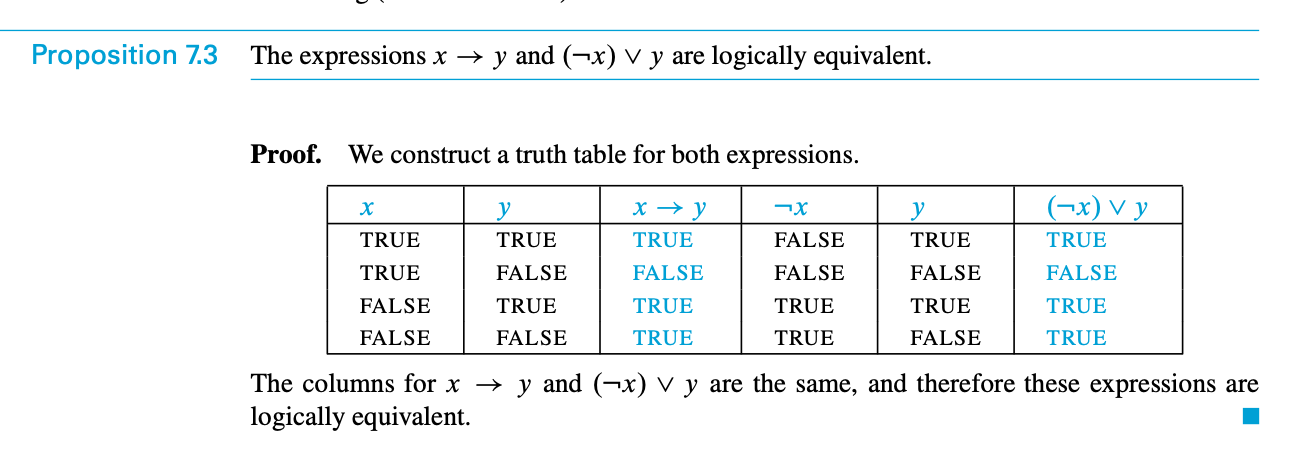
\includegraphics[width=\textwidth]{images/sec_7_reading_quiz_solution}
        \caption{Solution to Reading Quiz (Sec. 7)}
        \label{fig:figure1}
\end{figure}
\pause 
\vfill 
\begin{myredbox}[title=Scoring rubric]
\footnotesize 
\begin{itemize}
\item 10/10 points if truth tables for $x \implies y$ and $(\lnot x) \lor y$ were both given correctly, and \textit{there was some explanation of how the latter was determined.}
\item 7.5/10 points if truth tables for $x \implies y$ and $(\lnot x) \lor y$ were both given correctly.  	
\end{itemize}

\end{myredbox}

\end{frame}


\begin{frame}{Sec. 7 Reading Quiz Scores}

\begin{figure}[ht]
        \centering
        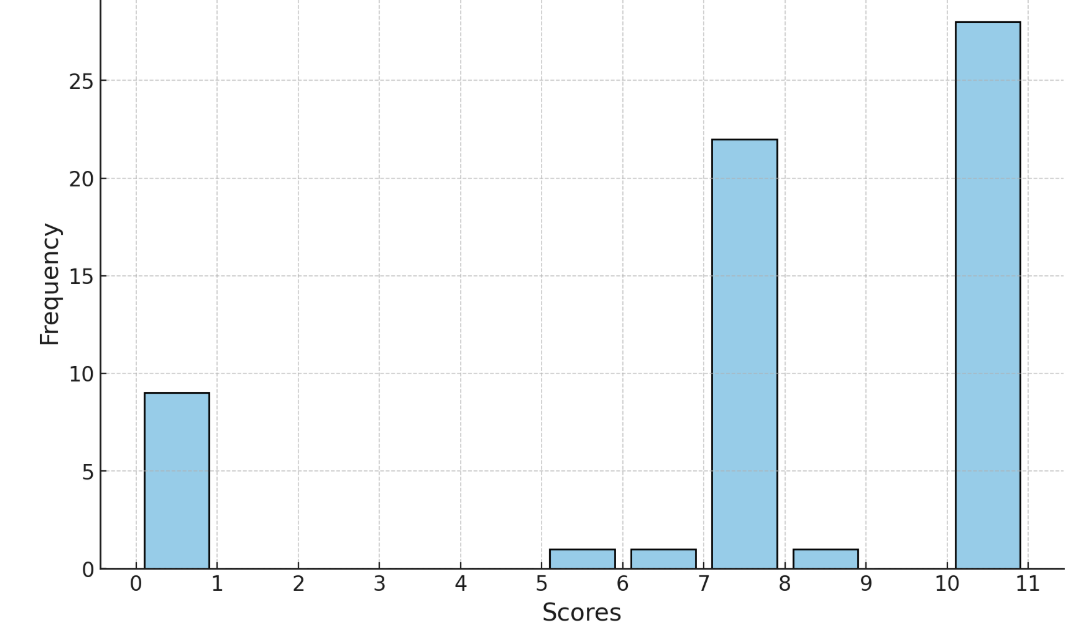
\includegraphics[width=.6\textwidth]{images/sec_7_reading_scores}
        \caption{Reading Quiz (Sec. 7)}
        \label{fig:figure2}
\end{figure}



\end{frame}


\begin{frame}{Group work}


\begin{myyellowbox}[title=Announcements about group work]
\begin{itemize}
	\item Ideas if you get stuck during group exercises:
	\begin{itemize}
	\item[(a)] Get my/Fatima's attention. 
	\item[(b)] Find other group to give a hint/lead.
	\item[(c)] Use textbook as resource.
	\end{itemize} 
	\item It's okay to get stuck! That's a \underline{natural} part of learning!
\end{itemize}	
\end{myyellowbox}
\vfill 
\begin{mygreenbox}[title=Quote of the Semester]
“The best way to learn is to do; the worst way to teach is to talk.” \\

-- Paul Halmos, a renowned mathematician and expositor
\end{mygreenbox}

\end{frame}


\begin{frame}[standout]

\alert{Group work (Boolean algebra)}
\vfill
Students are randomly assigned into groups of 3 on the next slide.
\vfill 
Each group gets $\half$ of a white board.
\vfill
If the  $\half$ white board is inconvenient, feel free to write on a window! 
\end{frame}




\begin{frame}
\footnotesize
Group 1: tyler.broesel,ryan.barrett2,jada.zorn\\
Group 2: jacob.ruiz1,mason.barnocky,jacob.ketola\\
Group 3: devon.maurer,peter.buckley1,cameron.wittrock\\
Group 4: alexander.knutson,delaney.rubb,peyton.trigg\\
Group 5: tristan.nogacki,jett.girard,anthony.mann\\
Group 6: evan.barth,owen.obrien,nicholas.harrington1\\
Group 7: connor.graville,luka.derry,pendleton.johnston\\
Group 8: lucas.jones6,william.elder1,luke.donaldson1\\
Group 9: lynsey.read,connor.yetter,blake.leone\\
Group 10: alexander.goetz,jakob.kominsky,samuel.mosier\\
Group 11: colter.huber,samuel.rollins,justice.mosso\\
Group 12: conner.reed1,jonas.zeiler,james.brubaker\\
Group 13: joseph.triem,bridger.voss,matthew.nagel\\
Group 14: julia.larsen,timothy.true,emmeri.grooms\\
Group 15: jacob.shepherd1,jack.fry,nolan.scott1\\
Group 16: michael.oswald,carsten.brooks,john.fotheringham\\
Group 17: evan.schoening,jeremiah.mackey,erik.moore3\\
Group 18: derek.price4,carver.wambold,aaron.loomis\\
Group 19: joseph.mergenthaler,yebin.wallace,adam.wyszynski\\
Group 20: samuel.hemmen,reid.pickert,griffin.short\\
Group 21: micaylyn.parker,sarah.periolat,zeke.baumann\\
Group 22: ethan.johnson18,connor.mizner,kaden.price, caitlin.hermanson\\
\end{frame}


\end{document}
